\documentclass{beamer}

\usepackage[utf8]{inputenc}

\input{../helper}
\graphicspath{{../img/}}

\title{Introdução à Computação \\ complexidade de algorítmos e notação O}
\author{Alexandre Rademaker}
\date{}

\begin{document}

\begin{frame}
 \maketitle
\end{frame}


\begin{frame}[fragile,allowframebreaks]{análise de algorítmos}

  Lembrando que quando implementamos \textbf{algorítmos}, queremos
  normalmente avaliar se eles estão corretos e terminam.
 
  Mas também normalmente queremos \textbf{eficiência} no uso dos
  \textbf{recursos}: tempo e memória.
 
  Mas então como comparar dois programas que fazem a mesma tarefa?
  Como estimar o 'tempo' necessário para uma determinada tarefa ser
  executada?

  Podemos também discutir a clareza do algorítmo (custo manutenção).
  
  \framebreak

  Podemos medir o tempo de processamento de cada implementação? Mas
  isso irá depender de cada máquina.

  \lstinputlisting[style=normalc,caption=src/sum.c]{src/sum.c}

  \framebreak

  \begin{lstlisting}[style=code]
    > time ./sum 10000000
    sum = 49999995000000
      0.02s user 0.00s system 5% cpu 0.402 total

    > time ./sum 100000000
    sum = 4999999950000000
      0.15s user 0.00s system 98% cpu 0.225 total

    > time ./sum 1000000000
    sum = 499999999500000000
      1.25s user 0.00s system 99% cpu 2.188 total
  \end{lstlisting}

  Chamamos de avaliação empírica. Diferenças podem ser consequência de
  fatores imprevisíveis, difícil replicação de resultados em
  diferentes máquinas.
  
\end{frame}


\begin{frame}[fragile,allowframebreaks]{complexidade dos algoritmos}

  \begin{center}
    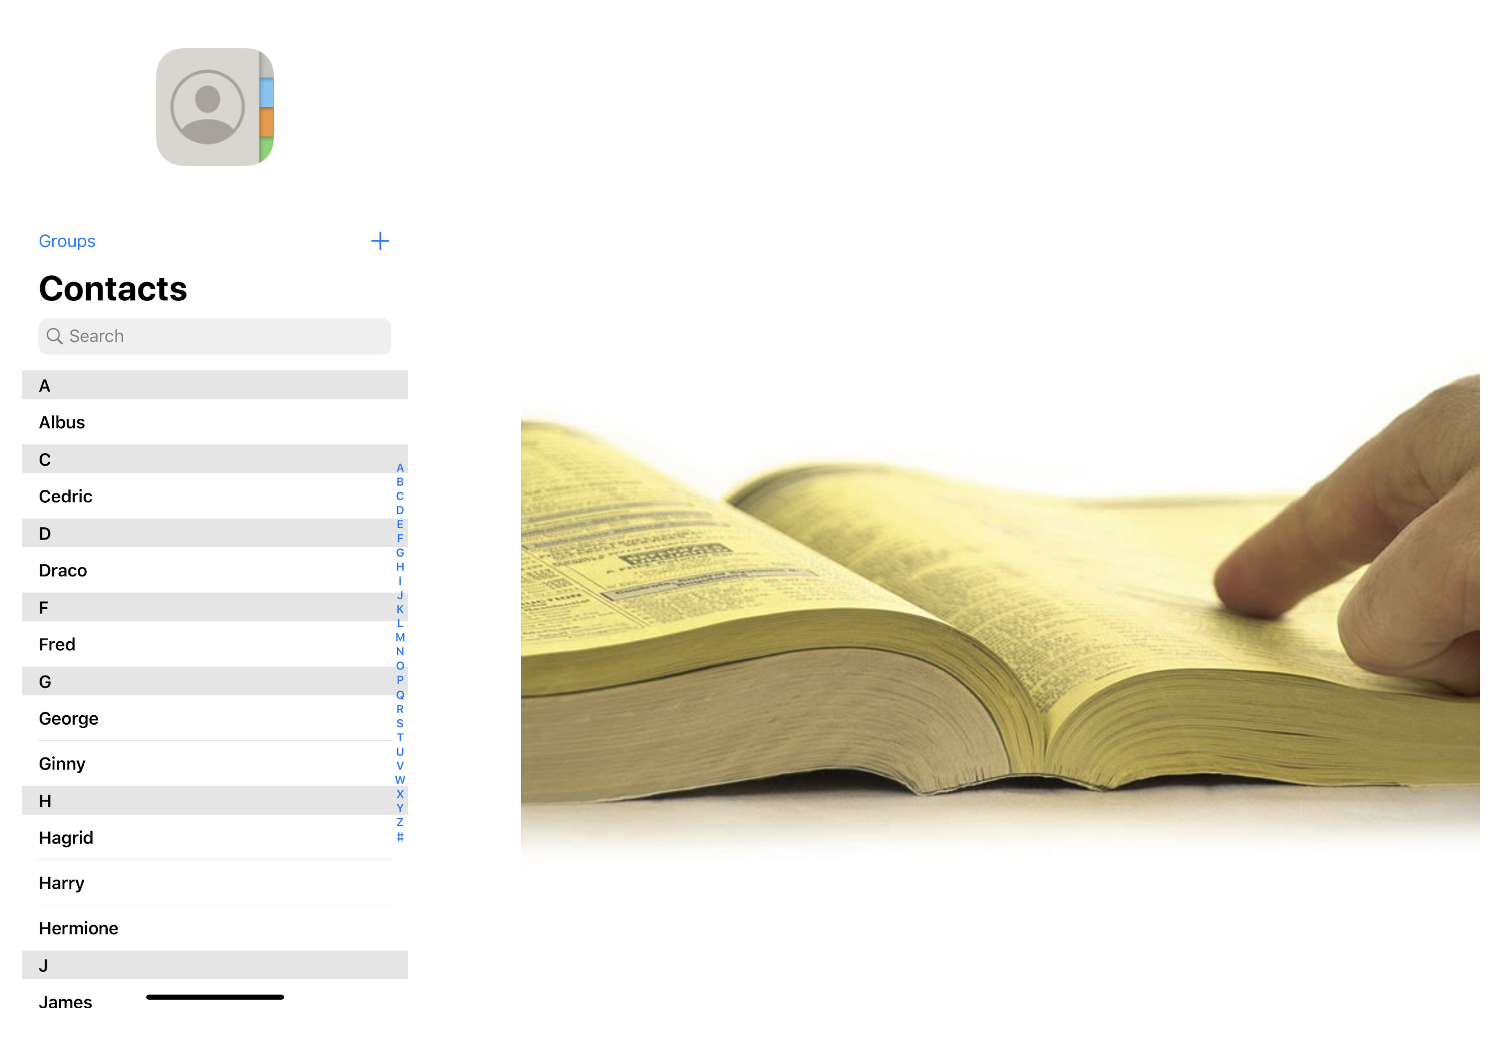
\includegraphics[width=.9\textwidth]{phonebook.png}
  \end{center}

  \framebreak

  busca por um nome:

  \begin{enumerate}
  \item Podemos abrir o livro e começar da primeira página, procurando
    um nome uma página de cada vez. {\color{red} Correto?}
  \item Podemos folhear o livro duas páginas de cada vez. {\color{red}
      Correto?}
  \item Abrir o livro no meio, decidir se nosso nome ficará na metade
    esquerda ou na metade direita (está em ordem alfabética) e
    escolher metade. {\color{red} Correto?}
  \end{enumerate}

  Um algorítmo deve ser uma
  \href{https://youtu.be/Ct-lOOUqmyY}{sequência precisa} de
  instruções!

  \framebreak
  
  Temos a busca {\color{red} de uma página por vez}, a busca
  {\color{yellow} de duas em duas páginas} e a busca {\color{green}
    binária}.

  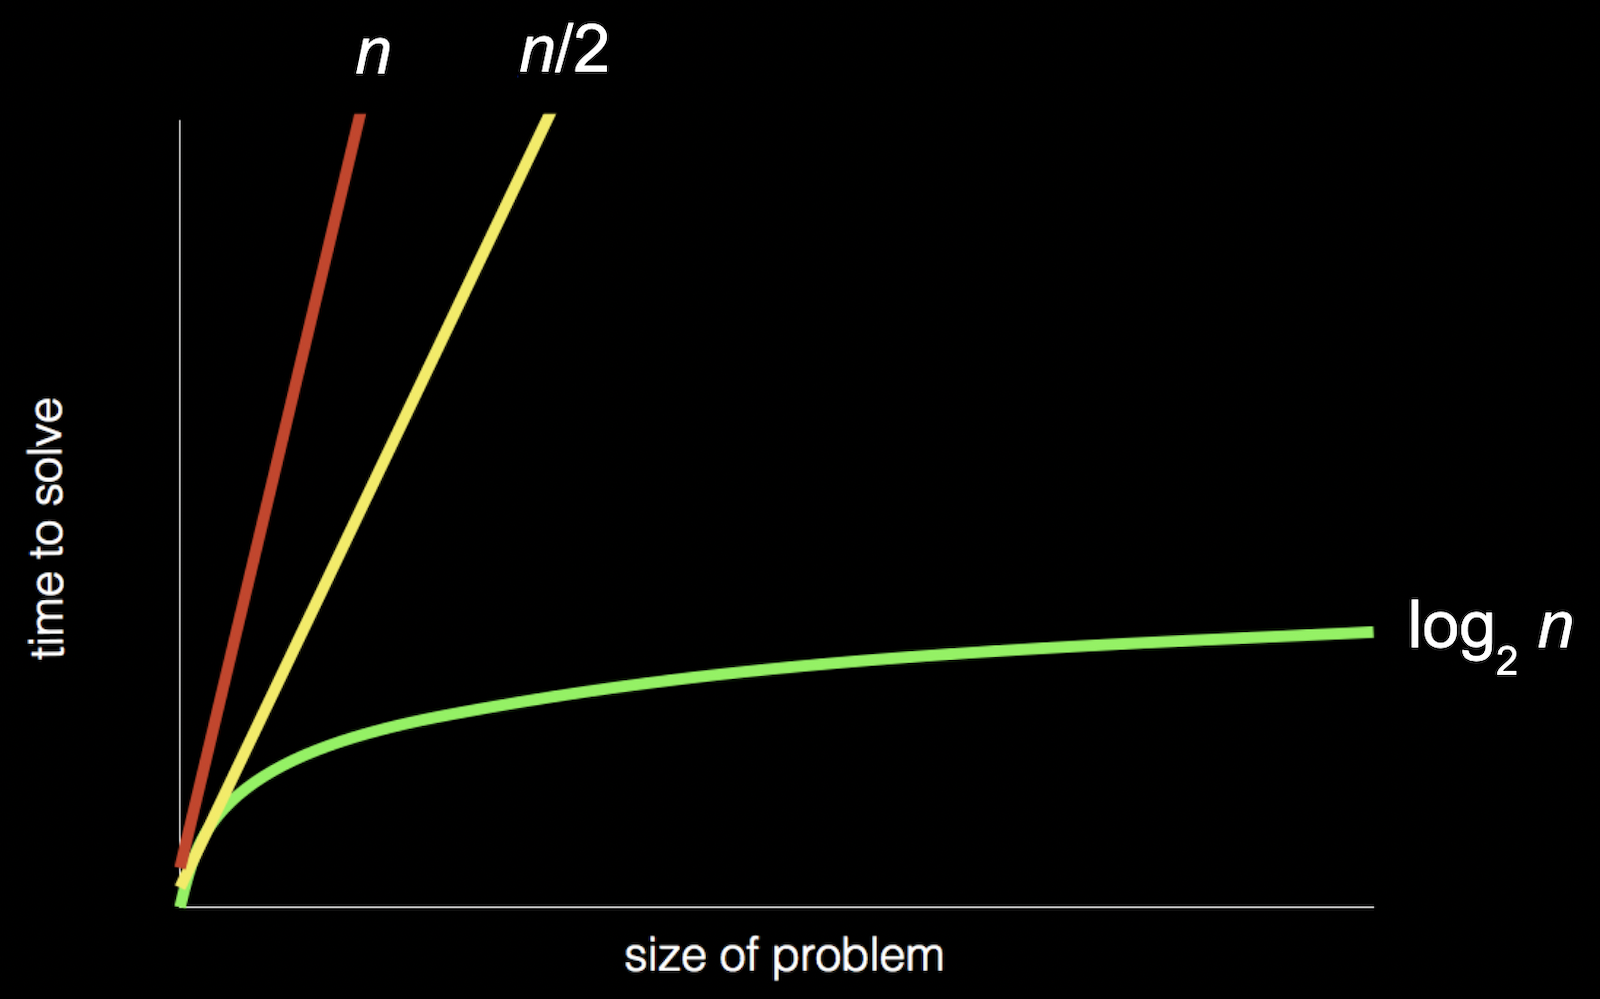
\includegraphics[width=.6\textwidth]{time_to_solve.png}

  \framebreak

  As linhas {\color{yellow} amarela} e {\color{red} vermelha} na
  verdade de comportam de forma bastante parecida para valores muito
  grandes de $n$.

  A linha {\color{green} verde} no entando, é bastante diferente, e
  descrita como $O(\log n)$, na ordem de $\log n$.

  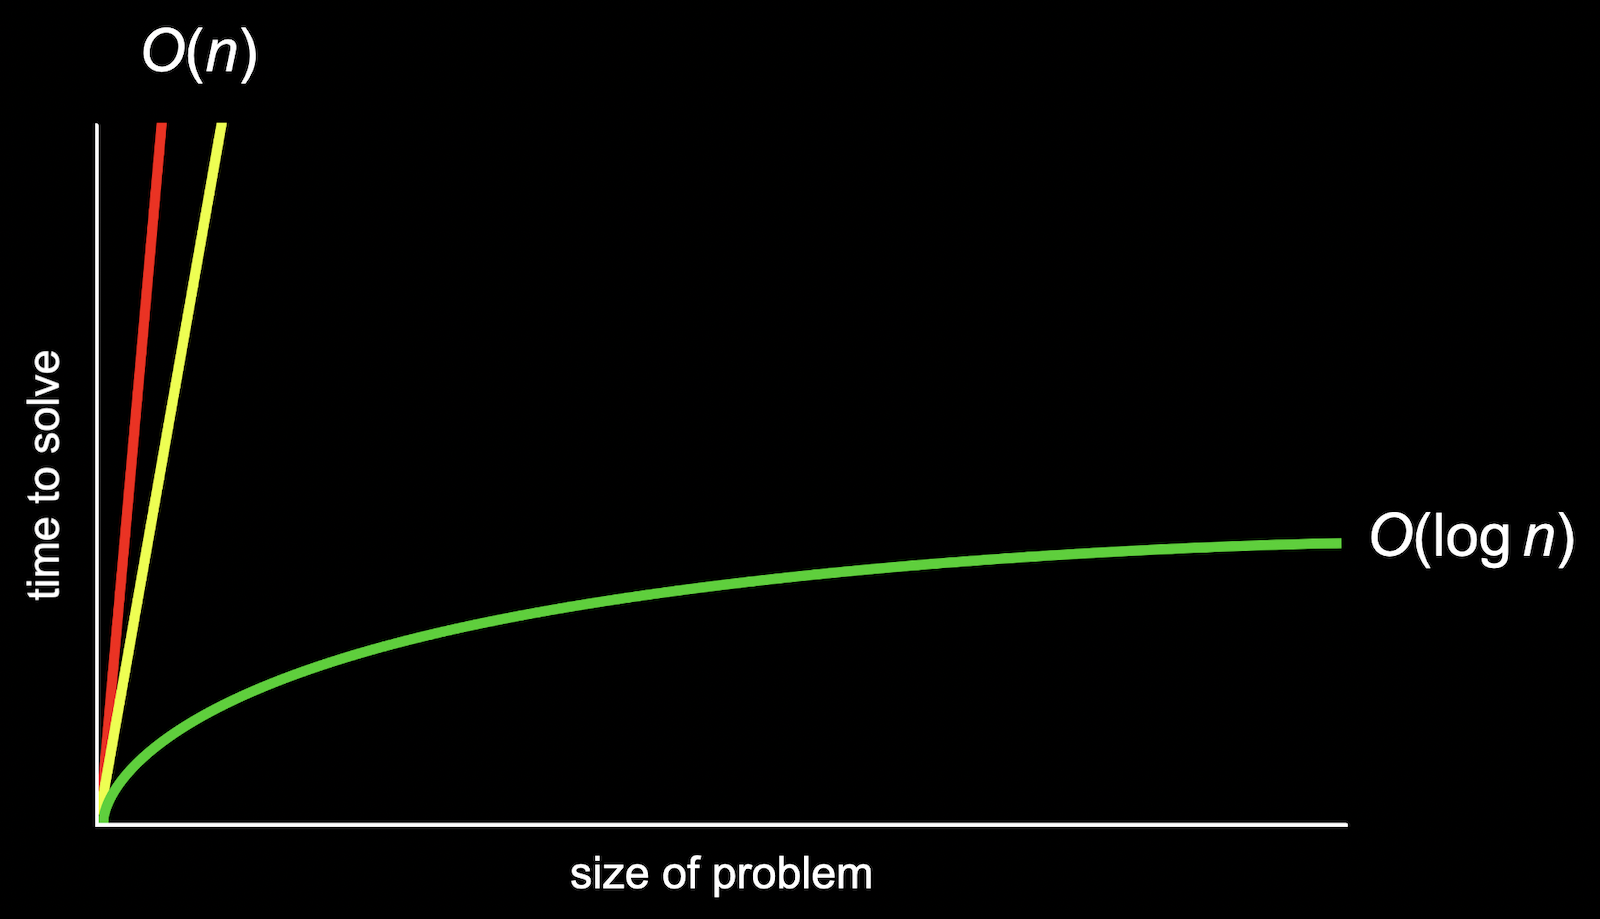
\includegraphics[width=.7\textwidth]{time_to_solve_zoomed_out.png}

  \framebreak

  A distinção entre fatores constantes (relacionados a velocidade do
  hardware, por exemplo) e o tempo de execução, à medida que o tamanho
  do problema aumenta, é de vital importância no estudo de algoritmos.

  A idéia principal medir o consumo do recurso (tempo mas pode ser
  também memória) como uma função, com o tamanho da entrada como
  parâmetro.

  \framebreak

  Podemos ter um programa com tempo de execução:
  \[
    T(n) = 2 n + 7
  \]

  Os valores irão geralemente representar o número de certas
  quantidades de instruções elementares. E a entrada pode ser a
  quantidade de itens tratados ou o número de bits necessários para
  representar a entrada.

\end{frame}  


\begin{frame}[fragile,allowframebreaks]{Notação $O$}  

  A notação $O$ é usada para descrever a complexidade de
  algorítmos. Diferentes algorítmos, para um mesmo problema, podem ter
  complexidades diferentes.

  Geralmente dizemos que um problema $P$ tem complexidade $C$ se o
  melhor algoritmo $A$ conhecido para resolver $P$ tem complexidade $C$.

  Com a notação $O$ falamos de complexidade sem precisar medir tempo
  de execução dos programas.
  
  \framebreak

  \begin{block}{Notação $f = O(g)$}
    Seja $f(n)$ e $g(n)$ funções de números inteiros positivos para
    reais positivos. Dizemos que $f = O(g)$ (que quer dizer que $f$
    não cresce mais rápido que $g$) se existe uma constante $c > 0$
    tal que $f(n) \leq c . g(n)$.
  \end{block}

  Então se $G(n)$ é a função que descreve a linha {\color{green}
    verde}, isto é, um algoritmo que para uma data entrada $n$ executa
  um número de passos não superiror à $\log n$, dizemos que $G$ é
  $O(\log n)$, ou $G = O(\log n)$, que sua complexidade é $O(\log n)$.

  \framebreak

  Para valores maiores que $n_0$, $T(n)$ é sempre menor que $cn^2$, logo
  dizemos que $T(n)$ é $O(n^2).$

  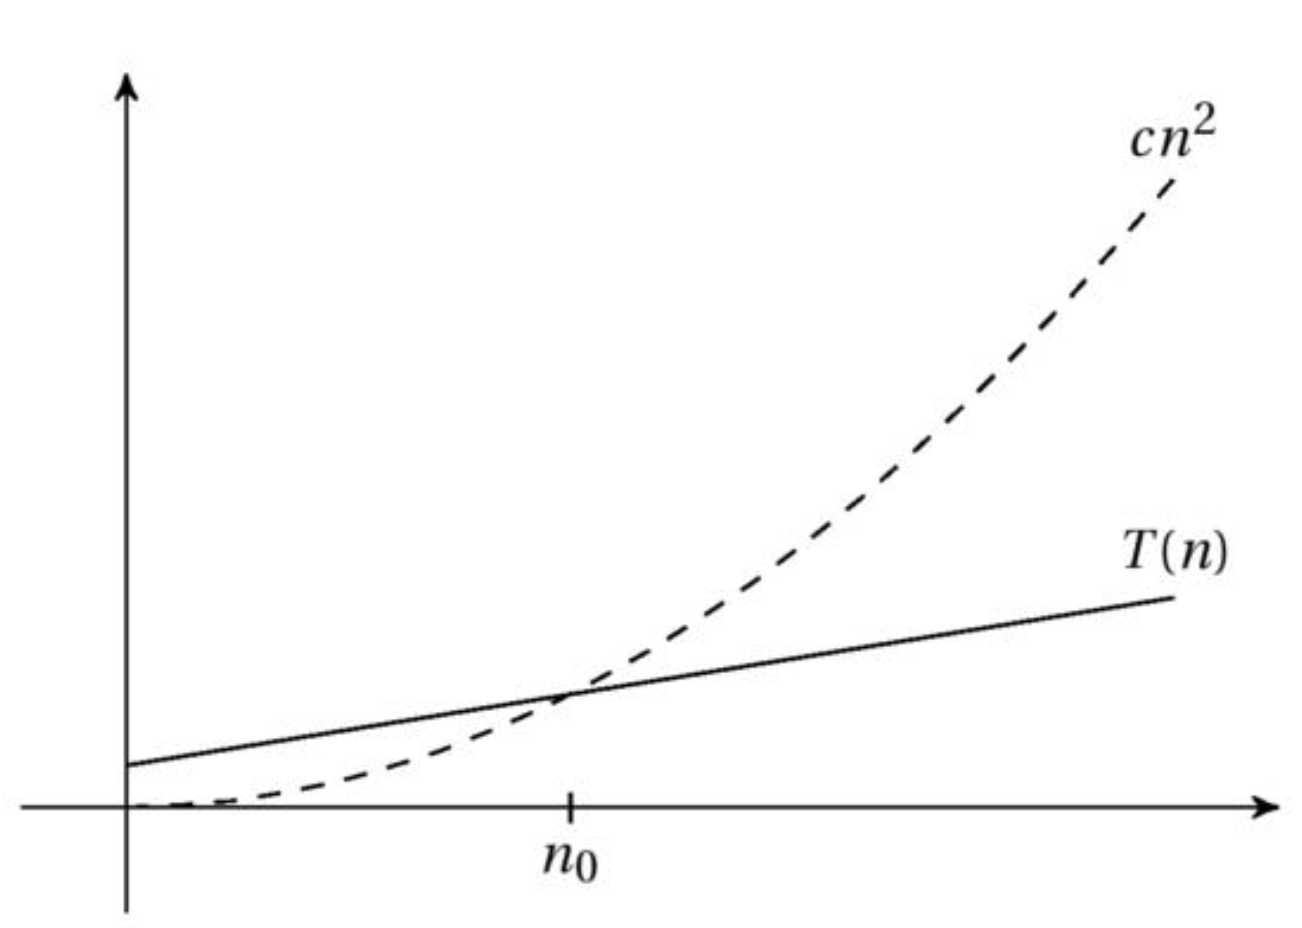
\includegraphics[width=.7\textwidth]{graph-asymptotic.png}

  \framebreak

  \begin{multline*}
    O(1) < O(\log n) < O(n) < O(n \log n) \\
    < O(n^2) < O(n^k) < O(k^n) < O(n!)
  \end{multline*}
  
  Algumas complexidades comuns são:

  \[
    O(n^2) \quad O(n \log n) \quad O(n) \quad O(\log n) \quad O(1)
  \]

  \framebreak

  Existe também a notação $\Omega$ para descrever o limite inferior do
  número de passos de um algorítmo.

  Quantos passos irá executar no \emph{melhor caso}.  A notação $O$,
  por outro lado, descreve quantos passos o algorítmo irá executar no
  \emph{pior caso}.

  E finalmente, temos a notação $\Theta$ para os casos onde o pior e
  melhor caso são os mesmos (limite inferior e superior iguais).

  \framebreak

  Embora as definições anteriores possam parecer complicadas, alguns
  conceitos são facilmente entendidos:

  Qualquer polinomial $n^k$ (qualquer expoente, mesmo fracionário)
  domina qualquer logarítmo $\log_a n$ (qualquer base).

  Qualquer exponencial domina qualquer polinomial. Logo $3^n$ cresce
  mais rápido $n^5$.

  \framebreak

  algumas regras práticas então:

  Em um polinômio, apenas a parcela com maior expoente
  importa, $\Theta(n^2 + n^3 + 42) = \Theta(n^3)$.

  Fatores constantes não importam,
  $\Theta(4.2 n \log n) = \Theta(n \log n)$.

  Para $\Omega$ e $O$, queremos manter o limite superior baixo e
  limite inferior alto. $n^2$ é tecnicamente $O(n^3)$.

  \framebreak

  Tecnicamente incorreto, dado que $O(n)$ é uma classe (conjunto) de
  funções, mas podemos dizer:

  \[
    \Theta(f) + \Theta(g) = \Theta(f + g)
  \]

  \[
    \Theta(f) . \Theta(g) = \Theta(f . g)
  \]
  
\end{frame}



\end{document}

%%% Local Variables:
%%% mode: latex
%%% TeX-master: t
%%% End:
